\documentclass[tikz,border=2pt]{standalone}
% Preámbulo común de los diagramas TikZ (misma paleta y letra que las notas)
\usepackage[T1]{fontenc}\usepackage[utf8]{inputenc}
\usepackage{libertinus}\usepackage{libertinust1math}
\usepackage[defaultsans,scale=0.92]{lato}
\usepackage{amsmath,amssymb,bm}
\usepackage{tikz}\usetikzlibrary{calc,positioning,arrows.meta,shapes.geometric,decorations.pathreplacing,decorations.pathmorphing,fit,backgrounds}
\definecolor{snlazul}{HTML}{1E5AA8}\definecolor{snlnoche}{HTML}{14213D}\definecolor{snlvioleta}{HTML}{6C4AB6}
\definecolor{snlcoral}{HTML}{D1495B}\definecolor{snlambar}{HTML}{E09F3E}\definecolor{snlverde}{HTML}{2A9D8F}
\definecolor{snlteal}{HTML}{0F7173}\definecolor{snlgris}{HTML}{5C677D}\definecolor{snlfondo}{HTML}{F4F6FA}
\tikzset{>={Stealth[length=2.2mm]},
  bloque/.style={draw=#1,fill=#1!8,thick,rounded corners=2pt,minimum height=11mm,minimum width=20mm,align=center,font=\small},
  bloque/.default=snlazul,
  suma/.style={draw=snlnoche,thick,circle,inner sep=0pt,minimum size=5mm},
  flecha/.style={->,thick,draw=snlnoche},
  etq/.style={font=\small,text=snlnoche},
  nota/.style={font=\footnotesize\sffamily,text=snlgris,align=center}}

\begin{document}
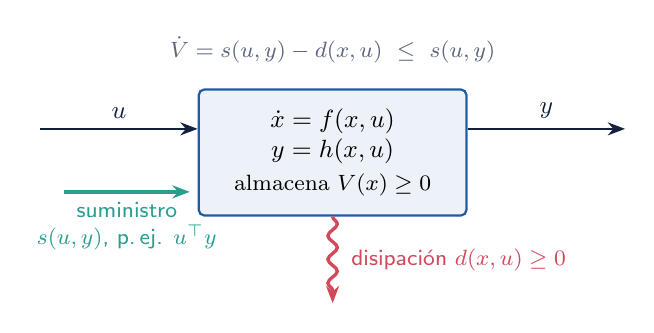
\begin{tikzpicture}
 \node[bloque=snlazul,minimum width=34mm,minimum height=16mm] (H) {$\dot x=f(x,u)$\\$y=h(x,u)$\\[1pt]{\footnotesize almacena $V(x)\ge0$}};
 \draw[flecha] ($(H.west)+(-20mm,3mm)$) -- node[above,etq]{$u$} ($(H.west)+(0,3mm)$);
 \draw[flecha] ($(H.east)+(0,3mm)$) -- node[above,etq]{$y$} ($(H.east)+(20mm,3mm)$);
 \draw[snlverde,very thick,->] ($(H.west)+(-17mm,-5mm)$) -- node[below,nota,text=snlverde]{suministro\\$s(u,y)$, p.\,ej. $u^\top y$} ($(H.west)+(-1mm,-5mm)$);
 \draw[snlcoral,very thick,->,decorate,decoration={snake,amplitude=.6mm,segment length=3mm,post length=1.5mm}] (H.south) -- node[right,nota,text=snlcoral]{\ disipación $d(x,u)\ge0$} ++(0,-11mm);
 \node[nota,above=2mm of H]{$\dot V = s(u,y)-d(x,u)\ \le\ s(u,y)$};
\end{tikzpicture}
\end{document}
